\documentclass[11pt,final]{article}%

% Page
\usepackage[margin=2.54cm, letterpaper]{geometry}
\usepackage{rotating}
\usepackage{epstopdf}
\usepackage{pdflscape}
\usepackage[english]{babel}
\usepackage[strict]{changepage}

% Math
\usepackage{amsthm,verbatim, amsmath, amsfonts, amssymb, mathtools, cases}
% \usepackage[toc, page, title, titletoc]{appendix}
\usepackage{type1cm}
\usepackage{bm}
\usepackage{courier}
\usepackage{relsize}
\usepackage{float}
% \usepackage{flafter}
\usepackage{graphicx}
% \usepackage[percent]{overpic}

% Tables & floats
\usepackage{tabularx, siunitx, tabu, array, longtable, multicol, booktabs,
	multirow, threeparttable}
\usepackage{siunitx}
\usepackage{ragged2e}
\usepackage[labelfont=bf,skip=0pt]{caption,subfig}
\usepackage[doublespacing]{setspace}
\usepackage{fancyhdr}
\usepackage{pageslts}
%\usepackage{endfloat}

% Quotes
\usepackage{dirtytalk}
% \usepackage{csquotes}

% Bibliography management
\usepackage{natbib}
\usepackage{har2nat}
\usepackage{breakcites}
\usepackage{xr-hyper}
\usepackage{hyperref}

% Cross-referencing
\usepackage{zref-xr,zref-user}
\zxrsetup{toltxlabel}
\zexternaldocument*{sup-material}

%\usepackage{nameref}
\usepackage[textsize=scriptsize,colorinlistoftodos, color=yellow]{todonotes}
% Allows using endfloat with sidewaystable (see endfloat doc)
% \DeclareDelayedFloatFlavor{sidewaysfigure}{figure}
% \DeclareDelayedFloatFlavor{sidewaystable}{table}

\setcounter{MaxMatrixCols}{30}
\providecommand{\U}[1]{\protect\rule{.1in}{.1in}}
\newcolumntype{C}{>{\centering\arraybackslash}X}
\newcolumntype{L}{>{\raggedright\arraybackslash}X}
\newcommand\mC[2]{\multicolumn{#1}{C}{#2}}
\newcommand{\vect}[1]{\bm{#1}} % \vector command
\geometry{verbose,headsep=0in}
\begin{document}

\section{Hypothesis}

When contagion is possible a bank failure negatively affects other banks probabilities of failures. As a result, bank failures rarely occur isolated but rather are clustered in time as shown below.

\begin{table}[]
    \centering
    \begin{tabular}{c}
         \textbf{USA}. Quarterly bank exits as a percentage of total banks in the quarter \\
         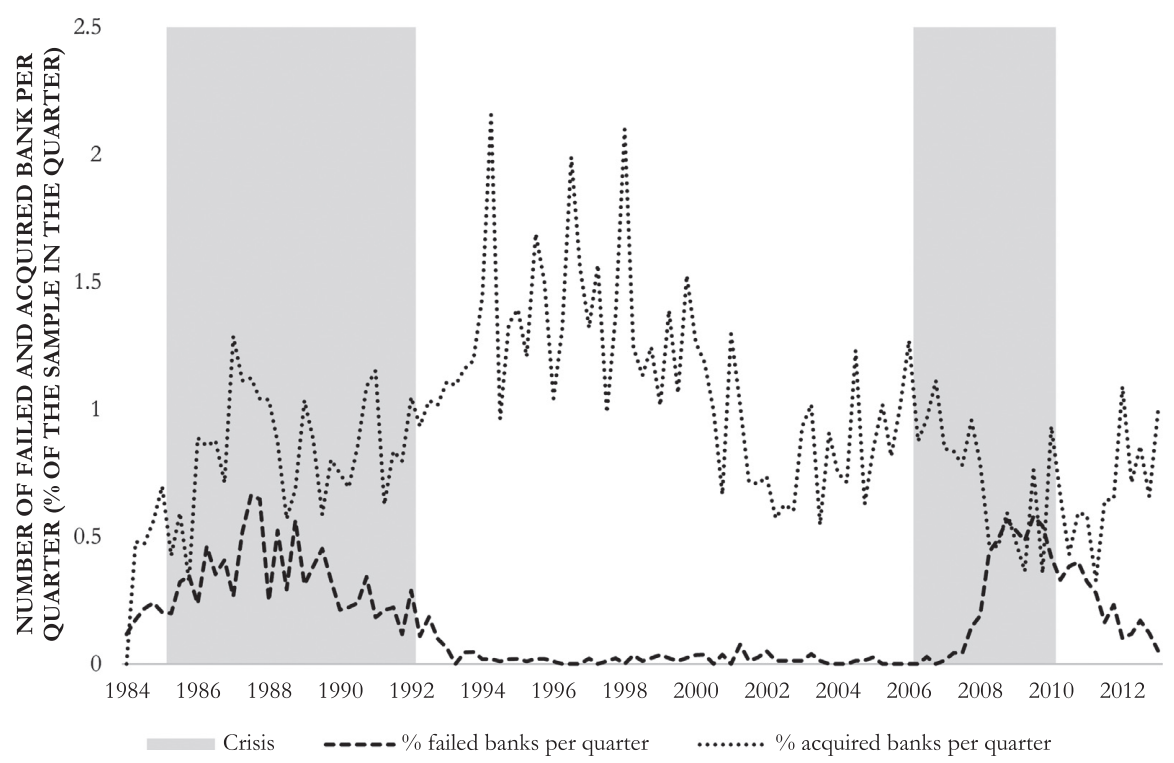
\includegraphics[width=\textwidth]{graphs/USA_Spokeviciute Keasey V Bank exits.png} \\
         Source: \cite{SpokeviciuteKeaseyVallascas2019} \\
        \addlinespace
          \textbf{Spain}. Banking crises in grey \\
         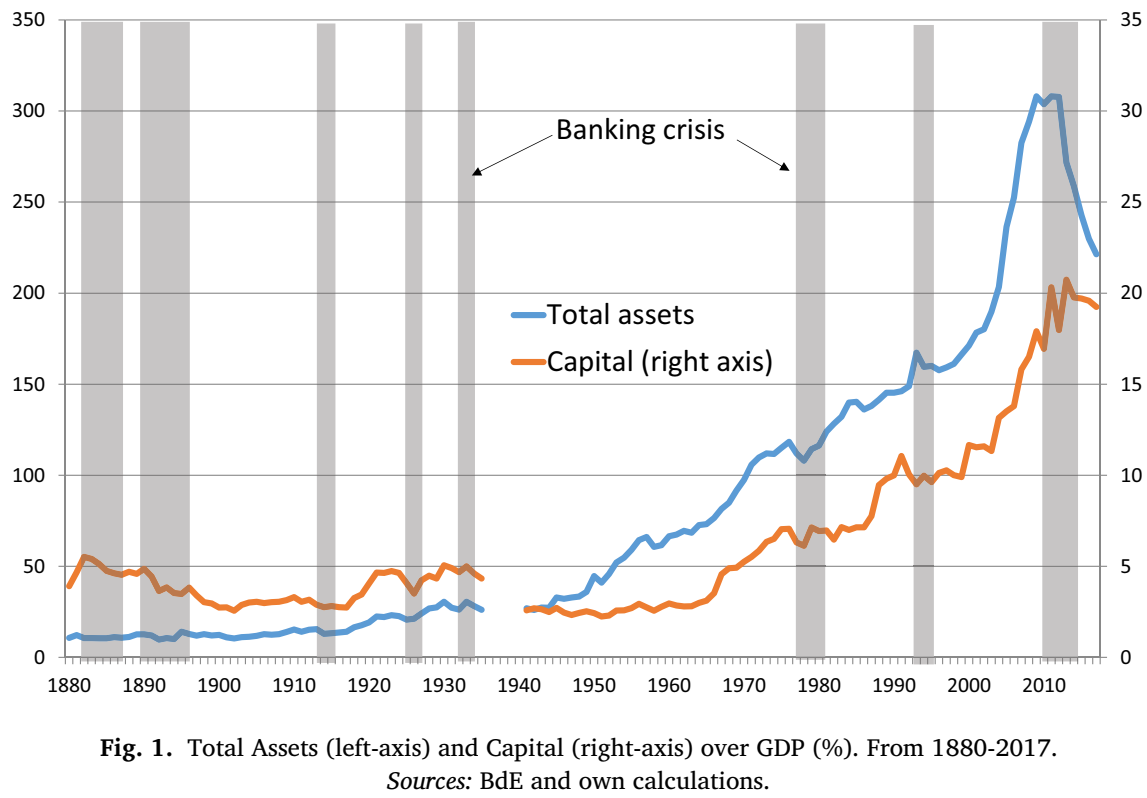
\includegraphics[width=\textwidth]{graphs/Spain banking crises.png}
          Source: \cite{BedayoEstradaSaurina2020} \\
    \end{tabular}
    \caption{Caption}
    \label{tab:my_label}
\end{table}

\section{Metodologhy}
\subsection{The spatial lag model of Elhorst Heijnen et al 2017}
The goal of the econometric model is to capture both aforementioned effects on a bank failure probability: the direct effect due to its own capital structure and the spillover effect. 

\subsubsection{Why survival models instead of logistic}
Survival models alow the probability of failure to increase over time. This relates to the lenght and severity of an economic crisis and bank abiity to withstand that shock: the longer a crisis is the more likely any given bank fails. Moreover, assuming a non-linear hazard function is related to the highly non-linear nonperomirng loans during crisis periods. 


The relation between the hazard rate and time is hihgli non-linear during a crisis. Consider for example the ratio of non-perfoming loans during crisis periods. From the figure, it is highly non-linear.

The treatment is the real sector crisis which start at the begnning of each sample and where at time $t=0$ all banks are alive, hence $S(0) = 1$. 

At each time $t$, bank $i$ can be in two states:
\begin{equation}
y_{i, t} =
\begin{cases}
	0 &	\text{Active at time }t, \\
    1 &	\text{Failed (bankruptcy or liquidation) at time }t, \\
\end{cases}
\end{equation}
Banks that fail at time $t$ are removed from the sample.  Denoted by $N^{0}_{t}$ active banks at time $t$ and $N^{1}_{t}$ failed banks by time $t$, the total number of banks is $N = N^{0}_{t} + N^{1}_{t}$.


A bank failure probability $y^{*}_{i,t}$ is not obvservablle but we observe failures at time $t$,  $y_{i,t}$. Define the unnobservable $N_{t}^{0} \times 1$ vector $\vect{y^{0*}_{t}}$ which contains the probability of failure of active banks at time $t$ and the $(N_{t}^{1} \times 1)$ vector $\vect{y_{t}^{1}}$ which fails at time $t$. The effect of bank failures in the second vector are intermediate by the 'distance' of the failing banks to the active banks.

The association among banks at time $t$  is captured by the spatial weight (or adjacency) matrix $W_{t}$:
\begin{equation}
W_{t} = 
\begin{bmatrix}
	0			&	w_{1, 2}	&	w_{1,3}		&	\cdots	&	w_{1, N}	\\
    w_{2,1}	&	0				&	w_{2,3}				&	\cdots	&	w_{2, N}	\\
    w_{3,1}	&	w_{3, 2}	&	0				&	\cdots	&	w_{3, N}	\\
    \vdots 	& \vdots		&	\vdots		&	\ddots	&	\vdots	\\
    w_{N,1}	&	w_{N, 2}	&	w_{N,3}		&	\dots	&	0	\\
\end{bmatrix},
\end{equation}

where the time subscript were omitted in the components of the matrix. 

One goal is capturing the effect that a that failure of a bank has on the 'neightbours' surviving banks. Thus in the model this matrix is divided into two submatrices: $W^{00}_{t}$for the relationships between active banks, and $W^{01}_{t}$ for the relationships between active banks and failed banks at time $t$. This division enable capturing the diffusion  effect of a failure: a fail banks affects its closest neighbours and this in turn reverberate in the system of active banks. 

Notice the dimesion of the adjacency matrix evolves over time. For each $t$, $W^{00}_{t}$ is $(N^{0}_{t} \times N^{0}_{t})$ and $W^{01}_{t}$ is $(N^{0}_{t} \times N^{1}_{t})$.

The capital ratio for each bank and all other indibidual covariates are stored by the $(N \times K)$ matrix $X$.

At each $t$ the failure probability of all active banks is updated based on the failures of that time and the covariates in $X$. 

The structural model is:
\begin{equation}
	\underbrace{\vect{y}^{0*}}_{N \times 1} = \alpha \vect{1} \,+\, \rho_{1}  W^{00}_{t} \vect{y}^{0*}_{t} \,+\, \rho_{2} W^{01}_{t} \vect{y^{1}_{t}}  \,+\, X_{t} \vect{\beta} \,+\, \vect{\epsilon^{0}}_{t}
    \label{eq:stc_form}
\end{equation}
where $\vect{1}$ is a vector of 1s, the $\vect{\epsilon}$ is a $N \times 1$ vector of idionsyncratic structural errors such that $\mathbb{E}(\vect{\epsilon} | \vect{x}, W)=0$. 
The parameters are the $N \times 1$ vectors $\alpha, \rho_1, \rho_2, \beta$ . 

The vector $\rho_1$ captures the interaction effect among active banks.  This interaction effect is an endogenous variable in equation (\ref{eq:stc_form}) since the variable $y_{t}^{0*}$ is unobservable. The parameter $\rho_2$ instead captures the interaciont of fail banks with active banks. $\beta$ captures the contribution of each bank own covariates to the failure probabilities of all banks. 

Solving for $\vect{y^{0*}}$ we obtain the reduced-form model,
\begin{equation}
\vect{y^{0*}} = (\vect{I} - \rho_1 \, W^{00}_{t} \, )^{-1} \vect{\alpha} \,+\, (\vect{I} - \rho_1 \, W^{00}_{t} \, )^{-1} \: \rho_{2} W^{01}_{t} \vect{y^{1}_{t}} \,+\, (\vect{I} - \rho_1 \, W^{00}_{t} \, )^{-1} \: X_{t} \vect{\beta}  \,+\, (\vect{I} - \rho_1 \, W^{00}_{t} \, )^{-1}   \vect{\epsilon^{0}}_{t}
\end{equation}
where $\vect{I}$ is the identifity matrix of order N.

Given enough macro controls (and fixed-effects?) we can mitigate any cross-correlation among panels such that $\mathbb{E}(\epsilon_{i} \epsilon_{j}) = 0$. 
A failed bank is not affected by alive banks. Once a bank failed, it is not affected by the outcome of healthy banks. Thus it makes sense to remove it from the sample.


\subsection{Marginal effects}
The coefficients from the above model cannot be interpreted as the marginall effects due to the nonlinearity of hte function . 

\cite{Elhorst2017} condier the marginal effect from the above model as:
\begin{align}
\Delta = \left( \frac{\partial \mathbb{E}[\vect{y_t}]  }{\partial x_{1k}} \, \cdots \, \frac{\partial \mathbb{E}[\vect{y_t}]  }{\partial x_{Nk}} \right) &= 
    \begin{bmatrix}
    \frac{\partial \mathbb{E}[\vect{y_{1,t}}]  }{\partial x_{1k}}	&	\cdots 	&	\frac{\partial \mathbb{E}[\vect{y_{1,t}}]  }{\partial x_{Nk}}	\\
    \vdots 	&	\ddots 	& \vdots  \\
    \frac{\partial \mathbb{E}[\vect{y_{N,t}}]  }{\partial x_{1k}}	&	\cdots 	&	\frac{\partial \mathbb{E}[\vect{y_{N,t}}]  }{\partial x_{Nk}}	
    \end{bmatrix} \\
&= diag[ \vect{\phi}	(\hat{\vect{y}}^{0}_{t}) ] \, (I - \rho_{1} W_{t}^{00})^{-1} \, I_{N} \beta_{k} 
\end{align}

\begin{align}
\Delta &=
    diag[ \vect{\phi}	(\hat{\vect{y}}^{0}_{t}) ] \,
    \begin{bmatrix}
    w^{-1}_{1,1} & w^{-1}_{1,2} &w^{-1}_{1,3} & \, \cdots \, & w^{-1}_{1,N} \\
    w^{-1}_{2,1} & w^{-1}_{2,2} &w^{-1}_{2,3} & \, \cdots \, & w^{-1}_{2,N} \\
    w^{-1}_{3,1} & w^{-1}_{3,2} &\ddots & \, \cdots \, & \vdots \\
    w^{-1}_{N,1} & w^{-1}_{N,2} &w^{-1}_{N,3} & \, \cdots \, & w^{-1}_{N,N} 
    \end{bmatrix}
    \begin{bmatrix}
    \beta_{k} & 0 & 0 & \, \cdots \, & 0 \\
    0 & \beta_{k} & 0 & \, \cdots \, & 0 \\
    0 & 0 & \, \ddots \, & \, \cdots \, & 0 \\
    0 & 0 & 0 & \, \cdots \, & \beta_{k} 
    \end{bmatrix} \\
&=
\begin{bmatrix}
    \textcolor{orange}{\phi_{1} (\hat{\vect{y}}^{0}_{1, t})}    &   0   &   \, \cdots \,    &   0 \\
    0    &   \textcolor{orange}{\phi_{2} (\hat{\vect{y}}^{0}_{2, t})}   &   \, \cdots \,    &   0 \\
    \vdots    &   0   &   \textcolor{orange}{\phi_{j} (\hat{\vect{y}}^{0}_{k, t})}    &   0 \\
    0    &   0   &   \, \cdots \,    &   \textcolor{orange}{\phi_{N} (\hat{\vect{y}}^{0}_{N, t})} 
\end{bmatrix}
\begin{bmatrix}
    \beta_k w^{-1}_{1,1} & \beta_k w^{-1}_{1,2} & \beta_k w^{-1}_{1,3} & \, \cdots \, & \beta_k w^{-1}_{1,N} \\
    \beta_k w^{-1}_{2,1} & \beta_k w^{-1}_{2,2} & \beta_k w^{-1}_{2,3} & \, \cdots \, & \beta_k  w^{-1}_{2,N} \\
    \beta_k w^{-1}_{3,1} & \beta_k w^{-1}_{3,2} & \ddots & \, \cdots \, & \vdots \\
    \beta_k w^{-1}_{N,1} &\beta_k  w^{-1}_{N,2} & \beta_k w^{-1}_{N,3} & \, \cdots \, & \beta_k w^{-1}_{N,N} 
\end{bmatrix} \\
&= 
\begin{bmatrix}
    \textcolor{orange}{\phi_{1} (\hat{\vect{y}}^{0}_{1, t})} \beta_k w^{-1}_{1,1} & \textcolor{orange}{\phi_{1} (\hat{\vect{y}}^{0}_{1, t})} \beta_k w^{-1}_{1,2} & \textcolor{orange}{\phi_{1} (\hat{\vect{y}}^{0}_{1, t})} \beta_k w^{-1}_{1,3}0 & \, \cdots \, & \textcolor{orange}{\phi_{1} (\hat{\vect{y}}^{0}_{1, t})} \beta_k w^{-1}_{1,N} \\
    \textcolor{orange}{\phi_{1} (\hat{\vect{y}}^{0}_{2, t})} \beta_k w^{-1}_{2,1} & \textcolor{orange}{\phi_{1} (\hat{\vect{y}}^{0}_{2, t})} \beta_k w^{-1}_{2,2} & \textcolor{orange}{\phi_{1} (\hat{\vect{y}}^{0}_{2, t})} \beta_k w^{-1}_{2,3}0 & \, \cdots \, & \textcolor{orange}{\phi_{1} (\hat{\vect{y}}^{0}_{2, t})} \beta_k  w^{-1}_{2,N} \\
    \textcolor{orange}{\phi_{1} (\hat{\vect{y}}^{0}_{3, t})} \beta_k w^{-1}_{3,1} & \textcolor{orange}{\phi_{1} (\hat{\vect{y}}^{0}_{3, t})} \beta_k w^{-1}_{3,2} & \ddots & \, \cdots \, & \vdots \\
    \textcolor{orange}{\phi_{1} (\hat{\vect{y}}^{0}_{N, t})} \beta_k w^{-1}_{N,1} &\textcolor{orange}{\phi_{1} (\hat{\vect{y}}^{0}_{N, t})} \beta_k  w^{-1}_{N,2} & \textcolor{orange}{\phi_{1} (\hat{\vect{y}}^{0}_{N, t})} \beta_k w^{-1}_{N,3} & \, \cdots \, & \textcolor{orange}{\phi_{1} (\hat{\vect{y}}^{0}_{N, t})} \beta_k w^{-1}_{N,N} 
\end{bmatrix}
\label{eq:full_def_marginal_effects}
\end{align}

where $\Delta$ is a N $\times$ N matrix,  $\vect{\hat{y^{0}_{t}}} = (I - \rho_{1} W_{t}^{00})^{-1} \, (\rho_{2} W_{t}^{01} \vect{y_{t}^{1}} \,+\, X_{t}^{0} \vect{\beta} )$ are the predicted values for $\vect{y}^{0}_{t}$.

The diagonal matrix $diag[ \vect{\phi}	(\hat{\vect{y}}^{0}_{t}) ]$ scales the diagonal elements of the $\tilde{S_r}$ matrix, which are the direct effects. 


The diagonal elements of the first-matrix contains where the off diagonal of the second-matrix. In other terms for bank 1, the effect of a change in bank 2 leverage is the second cell of the final matrix in the last line of (\ref{eq:full_def_marginal_effects}) given by:

\todo[inline]{Explain the average over time. We obtain this matrix for each t}

\todo[inline]{This is Girish's point. What you 'identify' as network effects is just the macro shock propagating through banks.}

\section{Estimation}
\subsection{The spatial lag probit model}
$\vect{y}^{*} = \rho W \vect{y}^{*} + X \vect{\beta} + \vect{\epsilon} $
$\vect{y}^{*} = (I - \rho W)^{-1} \: X \vect{\beta} \: +  (I - \rho W)^{-1} \vect{\varepsilon}$

$ \bm{\Omega} = \mathbb{E} \left[ \bm{\nu} \bm{\nu^{T}} \right]$


\subsubsection{Elhorst Heijnen et al 2017}
The problem is in this line
hessian(@(z)LikeliSALEISProbitcode(W,X,y,3,1000,z), ...
            [paramest(end); paramest(1:end-1)]);
The output matrix of this contains NaN and hence is not invertible. The function LikeliSALEISProbitcode(W,X,y,3,1000,z) converges and it works to estimate the parameters coefficients. 

\subsection{Inference about the marginal effect}

In an non-linear model, how does one build a confidence interval for the marginal effect?

I’m interested in the average marginal effect for variable $k$, defined as,  $\mathbb{E} \frac{\partial y}{\partial x_{k}} = N^{-1} \sum_{i=1}^{N} \phi(\vect{x}_{i} \vect{\hat{\beta}}) \: \hat{\beta_{k}})$ where $\phi(\cdot)$ is the Normal pdf and, $\hat{( \beta_{k}} - \beta_{0})\hat{\sigma_{k}} \sim \mathcal{N}(0,1)$ for $N>50$. 

Does $\mathbb{E} \frac{\partial y}{\partial x_{k}}$ follows a similar distribution to $\hat{\beta}$?

Can I build a 90\% confidence interval for $\mathbb{E} \frac{\partial y}{\partial x_{k}}$ as $\mathbb{E} \frac{\partial y}{\partial x_{k}} +/- 1.67 \: \hat{\sigma_{k}}$ ?

\subsection{Indirect and direct effects}
$ \mathbb{E} \left[ \frac{\partial y_{i}}{\partial x_{k, i}} \right] = (1-\rho)^{-1} \: \beta_{k}$

\subsection{valuing nodes}
Eisenberg & Noe (2001) demonstrate that, following an initial default in such a system, a unique vector that clears the obligations of all parties exists.
BALLESTER CALVO-ARMENGOL ZENOU 2006 Who is who in networks: develop the inetercentrality measure which measure what happens if you remove a node.

\section{Results}

\subsection{Size and systemic risk}
The figure below representes the interbank loans network for Argentinian financial entitites by December 1999. One interesting feature is that the relevance of a node in the network is not directly related to the size of the institution. Indeed, some medium or small financial institutions have a large number of linkages. This contradicts the idea of using the size of a financial institution as a measure of systemic risk. 

\subsection{1999}
\begin{itemize}
\item When considering only private banks banks alive at 1997q4, capital ratio is not different from zero.
\item \textbf{Network}. When using the average network till 1997q4 I don't get staistically significant results fro capital ratio nor for $\rho$ regardless of using $X_1999$ or $X_1998$. $W_{\sim 97q4}$ has far fewer links than $W_{\sim 98q4}$.
\item W and X contemporaneous. W ia verage till 98q4 and  is data during 1998. \url{A98_W98q4_creW_b97q4_s01q4}. No variable is significant at 15\% except for rho significant at 12\%. When using W till 1999q4 and X is annual average 1999 the result look better, see \url{A99_Wtill99q4_creW_b97q4_s03q4.html}. Revise this results because has more banks. 
\end{itemize}

\end{document}